\section{Sharp identification and the value of timing}\label{sec:identification}
\subsection{The information profile}
For a completion $u$, define
\begin{equation}\label{eq:profile}
 \Sprof_\Pi(u)=h(A+u)-T_\Pi-q(u,c-u),\qquad 0\le u\le c.
\end{equation}
When $c>0$, the terminal term is $c\,h(u/c)$; the mass form also covers $c=0$.

\begin{theorem}[Information profile, compatibility and sharpness]\label{thm:sharp}
For every valid observable law, $\Sprof_\Pi(u)=I(L;J_\Pi)$ under completion $u$. If $r>0$, its unique minimum on $[0,c]$ is attained at
\begin{equation}\label{eq:minimum}
 \ud=\frac{Ac}{r},\qquad \td=\frac{A}{r},\qquad
 \tau_\Pi=q(A,G)-T_\Pi.
\end{equation}
Here $\tau_\Pi=r I(L;J_\Pi\mid J_\Pi<\infty)$ is observable. The sharp identified set is
\begin{equation}\label{eq:sharp}
 \Thset_\Pi(\rho)=\{A+u:0\le u\le c,\ \Sprof_\Pi(u)\le\rho\}.
\end{equation}
It is empty for $\rho<\tau_\Pi$, a singleton $\{\td\}$ for $\rho=\tau_\Pi$, and a closed interval for $\rho>\tau_\Pi$. If $c=0$, the identified set is $\{A\}$ for $\rho\ge\tau_\Pi$, and is empty otherwise. If $r=0$, it is $[0,1]$ for every $\rho\ge0$.
\end{theorem}
\begin{proof}
Entropy decomposition gives $I(L;J_\Pi)=H(L)-H(L\mid J_\Pi)$, which is \eqref{eq:profile}. For $c>0$ and $0<u<c$, differentiation yields
\begin{align}
 \Sprof_\Pi'(u)&=\log\frac{u(G+c-u)}{(A+u)(c-u)},\label{eq:derivative}\\
 \Sprof_\Pi''(u)&=\frac{A}{u(A+u)}+
       \frac{G}{(c-u)(G+c-u)}>0\quad(r>0).\label{eq:curvature}
\end{align}
When $A,G>0$, the derivative vanishes exactly at $\ud$. When $A=0$ or $G=0$, the minimum is respectively the endpoint $0$ or $c$. Substitution gives $\Sprof_\Pi(\ud)=q(A,G)-T_\Pi$. This also follows from
\begin{equation}\label{eq:decomposition}
 I(L;J_\Pi)=I(L;R)+rI(L;J_\Pi\mid R=1),\qquad R=\ind\{J_\Pi<\infty\},
\end{equation}
where $I(L;R)$ is minimized at zero by making the unresolved harmful proportion equal to $A/r$. Continuity and strict convexity give the sublevel-set statements, including the limiting boundaries. Every admissible $u$ defines a joint table with rows $(a_1,\ldots,a_K,u)$ and $(b_1,\ldots,b_K,c-u)$, so every member of \eqref{eq:sharp} is attained; every joint law has this form. If $c=0$, the domain contains only $u=0$. If $r=0$, $J_\Pi$ is constant and its information is zero for any harmful proportion.
\end{proof}

Compatibility is therefore an observable restriction on $\rho$, although compatibility alone does not verify \eqref{eq:pis}. At its floor, the model selects the complete-case harmful proportion $\td$, rather than establishing that this proportion equals the true risk. At $K=1$, $T_1=q(A,G)$, $\tau_1=0$, and $\Sprof_1(u)=I(L;R)$: timing disappears but terminal selection remains subject to the budget. If $\rho\ge\log2$, the restriction is vacuous and the interval is $[A,A+c]$.

After an $O(K)$ accumulation of $A,G,T_\Pi$, each profile evaluation has constant cost. A compatible upper endpoint is $A+c$ if $\Sprof_\Pi(c)\le\rho$; otherwise it is obtained by bisection on $[\ud,c]$. The lower endpoint is analogous on $[0,\ud]$. Root-location precision $\varepsilon$ requires $O\{\log(1/\varepsilon)\}$ evaluations, with boundary cases handled directly. Population numerical endpoints are approximations to the sharp set; they are not substituted for conservative finite-sample bounds.

\subsection{Refinement as an exact information increment}
\begin{theorem}[Refinement and strict upper-risk improvement]\label{thm:refinement}
Let $\Pi_f$ refine $\Pi_c$ at the same terminal horizon, with fine masses summing to their coarse counterparts. For every completion $u$,
\begin{equation}\label{eq:shift}
 \Sprof_f(u)-\Sprof_c(u)=T_c-T_f
 =\tau_f-\tau_c=:\Delta\ge0.
\end{equation}
For $r>0$, $\Delta$ equals the conditional information $I(L;J_f\mid J_c)$ and is independent of $u$. It is positive exactly when a positive-mass resolved coarse band contains fine bands with different harmful proportions. Consequently,
\begin{equation}\label{eq:nesting}
 \Thset_f(\rho)\subseteq\Thset_c(\rho).
\end{equation}
If $c>0$, both sets are compatible, $\Delta>0$, and $\theta_{U,c}(\rho)<A+c$, then $\theta_{U,f}(\rho)<\theta_{U,c}(\rho)$.
\end{theorem}
\begin{proof}
The $A,G,c$ terms of \eqref{eq:profile} are unchanged by coarsening. Conditional entropy increases when resolved bands are merged, so $T_c-T_f\ge0$, with equality exactly under the stated within-band homogeneity condition by strict concavity of $h$. The conditional-information identity follows from the chain rule; the unresolved coarse category contains no finer split and contributes zero. Equation~\eqref{eq:nesting} follows by comparing sublevel sets. For strictness, the compatible coarse upper endpoint is above $\ud$ and below $c$ in hidden-mass coordinates, and has profile value $\rho$. Its fine profile value is $\rho+\Delta$, so it is excluded by the fine constraint. The fine feasible set is closed and nested, which makes its upper endpoint strictly smaller.
\end{proof}

For a partition and its endpoint coarsening, the identity is particularly transparent:
\begin{equation}\label{eq:effectivebudget}
 \Sprof_\Pi(u)=\tau_\Pi+\Sprof_1(u),\qquad
 \Thset_\Pi(\rho)=\Thset_1(\rho-\tau_\Pi)\quad(\rho\ge\tau_\Pi).
\end{equation}
The endpoint set on the right uses the same $A,G,c$. Thus timing deducts an observable amount from the information allowance for terminal selection. At equal excess budgets $\rho-\tau_\Pi$, common endpoint masses yield identical risk intervals; the information advantage is the one implied by a common absolute finest-path budget.

The total-information restriction accounts for both dependence expressed in resolved timing and dependence through terminal nonresolution. Under a common absolute budget, the observed timing contribution leaves less information available for terminal selection. This tightening is conditional on the total-budget assumption; it does not establish that selection among unresolved outcomes is weak. An application that instead fixes a separate allowance for terminal selection poses a different sensitivity question.

This is a fixed-budget comparison. Changing $\rho$ separately for each partition would mix information gain with a change in assumptions. Refinement can also increase $\tau$ above the declared budget. That outcome is model incompatibility, not successful risk certification. Conversely, positive timing information need not lower an upper endpoint that already saturates the worst-case bound at both resolutions.

\subsection{Certification geometry}
\begin{proposition}[Risk-budget frontier]\label{prop:safety}
Assume $r>0$ and compatibility. If $\beta<\td$, no choice of compatible $\rho$ certifies the risk. If $\beta\ge A+c$, every compatible budget certifies. In the remaining corridor $\td\le\beta<A+c$, define
\begin{equation}\label{eq:frontier}
 \rho_\Pi^*(\beta)=\Sprof_\Pi(\beta-A).
\end{equation}
Then certification is equivalent to $\tau_\Pi\le\rho\le\rho_\Pi^*(\beta)$. For nested partitions at a common $\beta$ in this corridor,
\begin{equation}\label{eq:frontiershift}
 \rho_f^*(\beta)-\rho_c^*(\beta)=\tau_f-\tau_c=\Delta.
\end{equation}
\end{proposition}
\begin{proof}
Every compatible set contains the minimum-information completion $\td$, and every completion has risk at most $A+c$. In the corridor, $\beta-A$ lies on the nondecreasing branch of the strictly convex profile. Its sublevel-set upper endpoint is at most this point exactly when $\rho\le\Sprof_\Pi(\beta-A)$. Compatibility supplies the lower bound on $\rho$. The shift is \eqref{eq:shift} evaluated at $\beta-A$.
\end{proof}

The frontier shift gives a decision interpretation of timing information. Provided the fine model is compatible, budgets above the endpoint frontier and below the fine frontier permit a fine certificate but exclude an endpoint certificate. A smaller upper bound matters operationally only if it crosses the chosen $\beta$.

\begin{figure}[!htbp]
\centering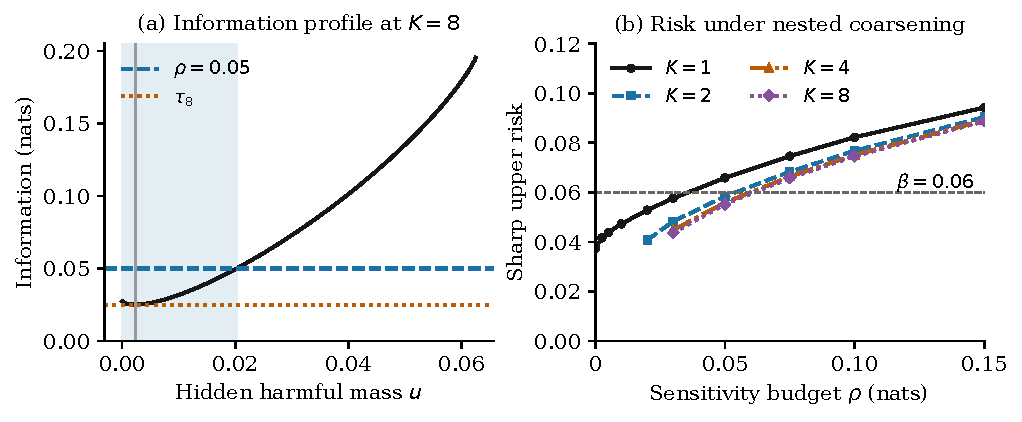
\includegraphics[width=\linewidth]{figures/identification.pdf}
\caption{Population information geometry for the timing-and-terminal harmful-late law ($\theta=0.05$, $q_1=0.30$, $q_0=0.05$, $\lambda_1=0.45$, $\lambda_0=-0.15$). (a) Eight-band information profile on a 1,001-point grid. Shading marks the compatible hidden masses at $\rho=0.05$; the vertical line marks $\ud$. (b) Sharp upper risks at the evaluated sensitivity budgets, under nested coarsenings of one eight-band law. The horizontal line is $\beta=0.06$. Incompatible values are absent; joining segments guide the eye and are not additional evaluations.}\label{fig:identification}
\end{figure}

\FloatBarrier
